\documentclass[10pt]{article}
\usepackage[margin=1in]{geometry}
\usepackage{graphicx}
\usepackage{booktabs}
\usepackage{amsmath}
\usepackage{hyperref}
\usepackage{float}
\usepackage[font=small,labelfont=bf]{caption}
\usepackage{parskip}
\usepackage{microtype}

\hypersetup{colorlinks=true, linkcolor=blue, urlcolor=blue}

\setlength{\parskip}{0.45em}
\setlength{\parindent}{0em}
\setlength{\textfloatsep}{8pt plus 2pt minus 2pt}
\setlength{\floatsep}{6pt plus 2pt minus 2pt}
\setlength{\intextsep}{6pt plus 2pt minus 2pt}

\makeatletter
\renewcommand\section{\@startsection{section}{1}{\z@}%
  {-2.5ex plus -1ex minus -.2ex}{1.5ex plus .2ex}{\normalfont\Large\bfseries}}
\renewcommand\subsection{\@startsection{subsection}{2}{\z@}%
  {-2ex plus -0.5ex minus -.2ex}{1ex plus .2ex}{\normalfont\large\bfseries}}
\makeatother

\title{\textbf{Assignment 3: Transformer is All You Need}\\[0.3em]
\large Tiny Shakespeare Next-Token Model (From-Scratch Transformer)}
\author{Andy Zhang}
\date{}

\begin{document}
\maketitle

\noindent\textbf{Code:} \url{https://github.com/zz3231/COMS4995-Applied-Machine-Learning-HW/tree/main/HW3}

\section{Introduction}

This report describes a \textbf{minimal causal Transformer} language model implemented in PyTorch for \textbf{next-token prediction} on the Tiny Shakespeare corpus. The training objective is standard causal LM: maximize $\log p(x_t \mid x_{<t})$ at each position using cross-entropy. We report \textbf{validation perplexity} $\mathrm{PPL} = \exp(\mathcal{L})$, where $\mathcal{L}$ is mean validation cross-entropy in nats; lower is better.

The model uses two Transformer blocks, $d_{\mathrm{model}}=128$, eight heads, feed-forward width $512$, \textbf{RMSNorm}, \textbf{sinusoidal positional encodings}, and \textbf{causal} multi-head self-attention. Tokenization is \textbf{Byte-Pair Encoding} with vocabulary size capped at \textbf{500}, fitted \textbf{only on the training split} after an 80/20 character-level partition so validation tokens do not influence merge statistics.

\section{Methods}

\subsection{Data and tokenization}

Tiny Shakespeare is loaded from the usual Karpathy URL ($\sim$1.1M characters). The first 80\% of characters are \texttt{train\_text}; the rest is \texttt{val\_text}. A ByteLevel BPE tokenizer (\texttt{tokenizers}) is trained on \texttt{train\_text} with \texttt{vocab\_size}=500 and \texttt{min\_frequency}=2. Overlapping windows of \textbf{65} tokens with stride \textbf{32} yield $\sim$12.8k training windows; each window yields \textbf{64} supervised positions (input = positions $0{:}T{-}1$, target = positions $1{:}T$).

\subsection{Model architecture}

We use \textbf{pre-LN} blocks: $x \leftarrow x + \mathrm{Dropout}(\mathrm{Sublayer}(\mathrm{RMSNorm}(x)))$ for attention and FFN sublayers. \textbf{Causal self-attention} applies a lower-triangular mask before softmax so query $i$ cannot attend to keys $j>i$. \textbf{Sinusoidal} positional vectors are added to token embeddings (scaled by $\sqrt{d_{\mathrm{model}}}$). A final RMSNorm and linear \textbf{language-model head} map hidden states to vocabulary logits. Total parameter count is on the order of one million, small enough for a laptop CPU or a single Colab GPU.

\subsection{Training and evaluation}

Optimization uses \textbf{AdamW} (learning rate $3\times 10^{-4}$, weight decay $0.01$), batch size \textbf{32}, dropout $0.1$, and \textbf{gradient clipping} (global norm 1.0). The main model trains for \textbf{25} epochs. Random seeds are fixed; validation uses \texttt{torch.no\_grad()}. Metrics are mean cross-entropy and $\mathrm{PPL}=\exp(\mathrm{CE})$ on the validation loader.

\subsection{Extra experiments}

\textbf{(A) Positional encoding ablation:} the same architecture without sinusoidal PE is trained for \textbf{15} epochs. Figure~\ref{fig:ablate} plots validation PPL for the first 15 epochs of the main run versus all 15 epochs of the no-PE model (aligned $x$-axis, fair epoch-matched comparison).

\textbf{(B) Shorter context:} datasets use block size \textbf{33} and stride \textbf{16} (32 prediction positions). A fresh model trains for \textbf{12} epochs. This run is \textbf{not} directly comparable to the main model (different sequence length $T$, different number of epochs, and a separate weight initialization); it illustrates the context-length versus compute tradeoff.

\section{Results}

\subsection{Training curves and perplexity}

Figure~\ref{fig:loss} shows training and validation cross-entropy and validation perplexity. Training CE decreases smoothly to $\approx 3.38$ by epoch 25; validation CE ends at \textbf{3.7217}, giving $\mathrm{PPL}=\textbf{41.33}$.

\begin{figure}[H]
\centering
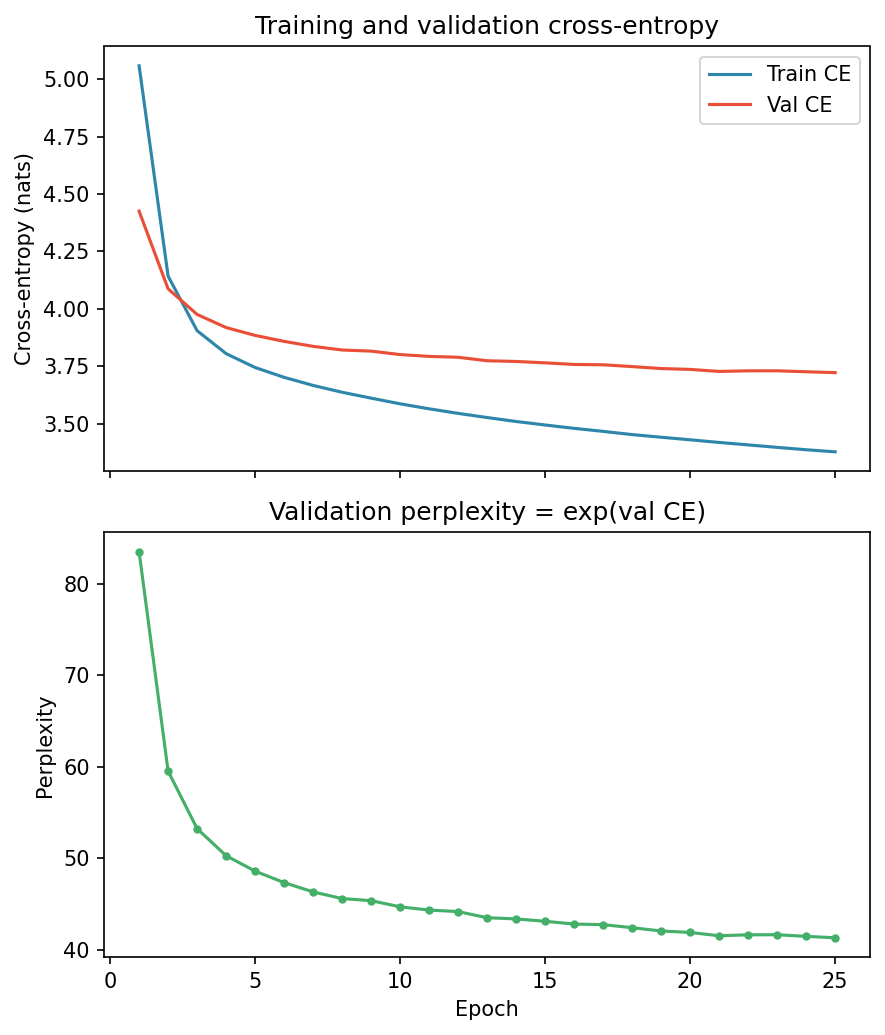
\includegraphics[width=0.72\textwidth]{fig_01_loss_ppl.png}
\caption{Training/validation cross-entropy (top) and validation perplexity (bottom) over 25 epochs.}
\label{fig:loss}
\end{figure}

\begin{table}[H]
\centering
\caption{Hyperparameters and reported metrics (from the submitted notebook run).}
\begin{tabular}{@{}ll@{}}
\toprule
Setting & Value \\
\midrule
Vocab & 500 BPE (train-only) \\
Block / stride (main) & 65 / 32 (64 positions) \\
Batch size & 32 \\
$d_{\mathrm{model}}$, layers, heads, FFN & 128, 2, 8, 512 \\
Optimizer & AdamW, lr=$3\times 10^{-4}$, wd=$0.01$ \\
Gradient clipping & max norm 1.0 \\
Main training & 25 epochs \\
Final train CE / val CE / val PPL & 3.38 / 3.72 / \textbf{41.33} \\
No-PE ablation & 15 epochs; final val PPL \textbf{43.58} \\
Short context & block 33, 12 epochs; final val PPL \textbf{40.19} \\
\bottomrule
\end{tabular}
\end{table}

\subsection{Attention heatmaps}

Heatmaps use one \textbf{validation} prefix (decoded ByteLevel subwords on both axes). The mask enforces a \textbf{strictly lower-triangular} pattern: each row (query position) has nonzero mass only on columns $\leq$ that index.

\paragraph{Layer 0, head 0 (Figure~\ref{fig:att1}).}
The early-layer map is relatively \textbf{diffuse} along allowed past positions: several predecessors receive moderate weight rather than a single sharp peak. Some mass concentrates on the most recent tokens (a local ``recency'' bias), which is typical when the model begins combining raw subword identities before higher-level structure is explicit.

\paragraph{Layer 1, head 2 (Figure~\ref{fig:att2}).}
The deeper head shows \textbf{sparser}, more peaked assignments on a subset of prior subwords. Different heads can specialize (e.g., attending to separators, frequent fragments, or specific predecessors); comparing L0H0 and L1H2 on the \textbf{same} sequence makes head diversity visible without conflating sample noise.

We did \textbf{not} re-render attention at early training epochs; all heatmaps are from the \textbf{converged} main model, so we cannot claim time-lapse evolution of attention within this report.

\begin{figure}[H]
\centering
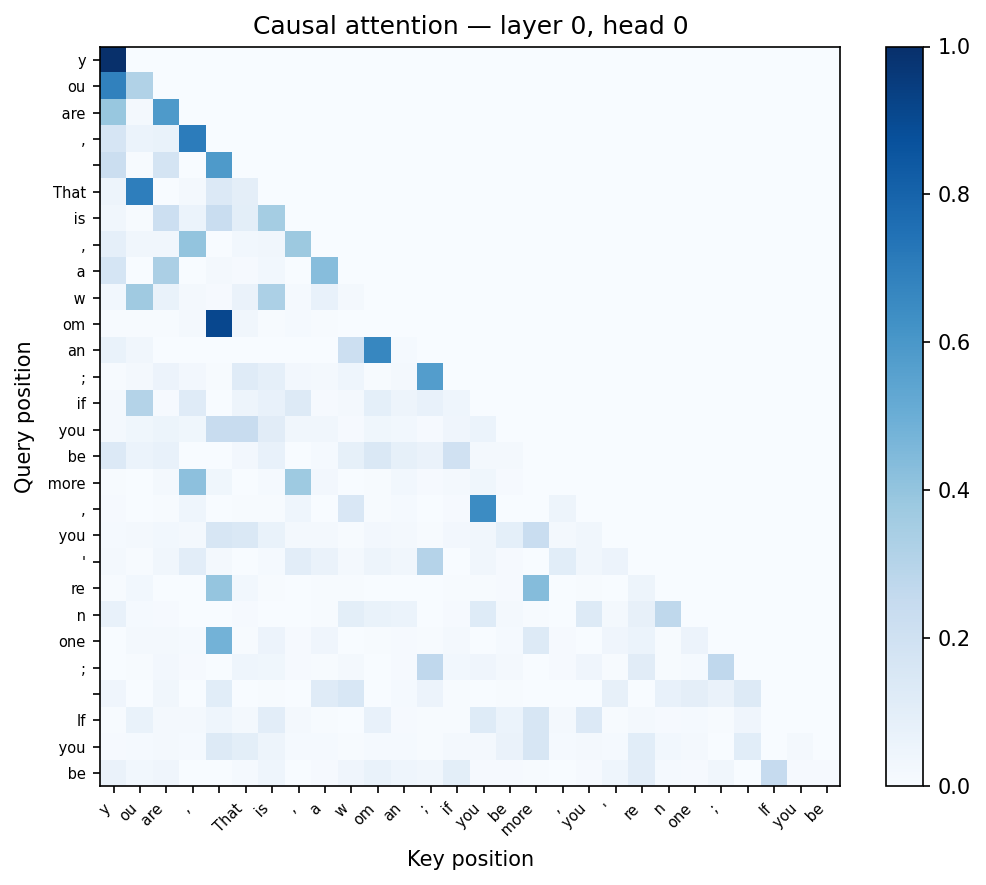
\includegraphics[width=0.75\textwidth]{fig_02_attention_L0H0.png}
\caption{Layer 0, head 0: causal attention on a fixed validation prefix (subword labels).}
\label{fig:att1}
\end{figure}

\begin{figure}[H]
\centering
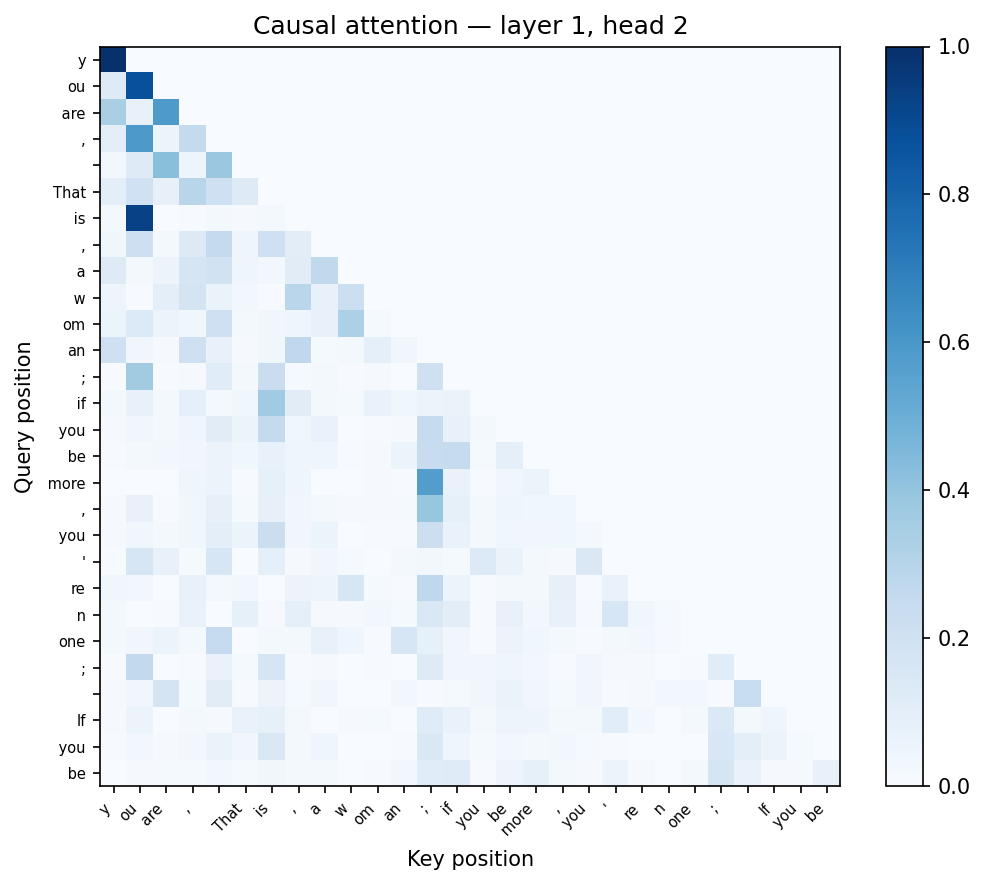
\includegraphics[width=0.75\textwidth]{fig_03_attention_L1H2.png}
\caption{Layer 1, head 2: same prefix as Figure~\ref{fig:att1}; sparser peaks than the early-layer head.}
\label{fig:att2}
\end{figure}

\subsection{Ablations and context length}

Figure~\ref{fig:ablate} shows that removing sinusoidal PE \textbf{raises} validation PPL at the same epoch index: after 15 epochs, no-PE reaches \textbf{43.58} versus \textbf{43.13} for the main model at epoch 15 (and \textbf{41.33} after the full 25-epoch main run). The gap supports the view that absolute position cues help even on this small model and corpus.

Figure~\ref{fig:short} gives validation PPL for the short-context setup. The final value \textbf{40.19} is \textbf{not} a claim that shorter context beats the main model overall---training length and $T$ differ. The intended takeaway is \textbf{operational}: shorter $T$ reduces attention memory and FLOPs (both scale roughly as $O(T^2)$ in this implementation) at the cost of less context for long-range dependencies.

\begin{figure}[H]
\centering
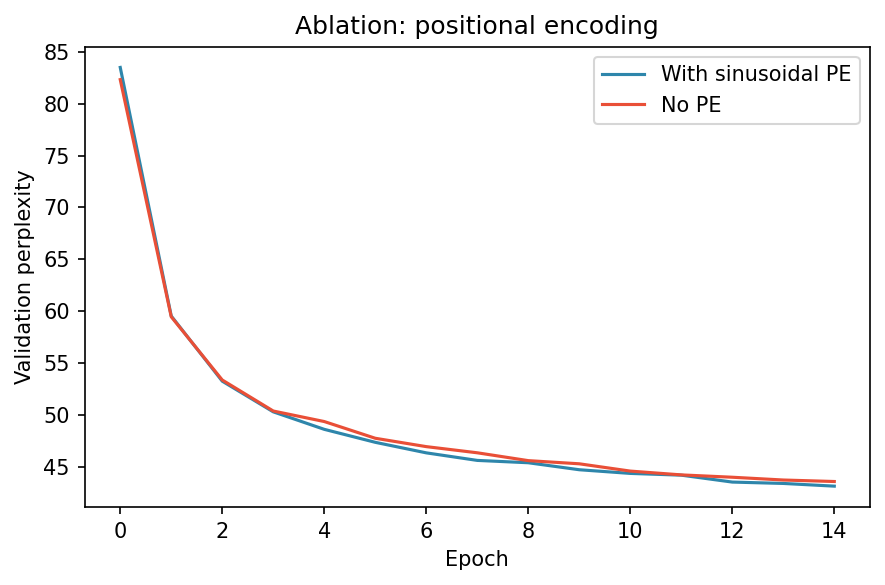
\includegraphics[width=0.62\textwidth]{fig_04_ablation_pe.png}
\caption{Positional encoding ablation: validation PPL for epochs 1--15, main model (truncated) vs.\ no-PE model.}
\label{fig:ablate}
\end{figure}

\begin{figure}[H]
\centering
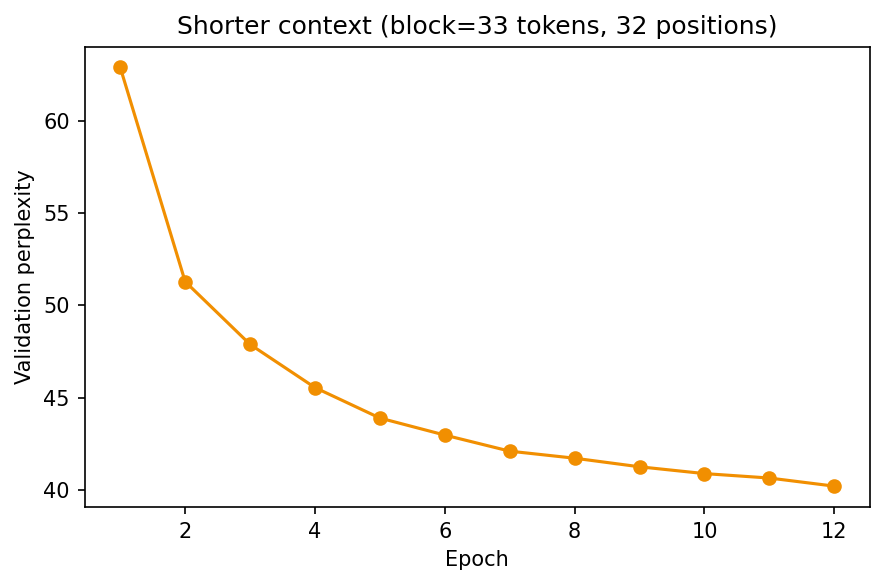
\includegraphics[width=0.62\textwidth]{fig_05_short_context.png}
\caption{Shorter context (block 33, stride 16): validation PPL over 12 epochs.}
\label{fig:short}
\end{figure}

\subsection{Qualitative generation (optional)}

We sampled text from the trained model with temperature $\approx 0.85$. Output is Shakespeare-\emph{flavored} but not coherent prose, e.g.\ fragmented lines such as ``That is, a woman; if you be more, you'er's thereock,'' mixed with stage-like labels. This matches expectations for a tiny model and limited training budget.

\section{Discussion}

\textbf{Stability.} In development, the most sensitive knobs were learning rate and gradient clipping; without clipping, loss occasionally spiked. Batch size 32 and AdamW defaults proved stable for 25 epochs.

\textbf{Positional information.} The ablation gives concrete evidence that sinusoidal PE improves validation PPL relative to an otherwise identical stack, consistent with the idea that self-attention is permutation-invariant in the absence of position tags.

\textbf{Memory and runtime.} For batch $B$, heads $H$, and sequence length $T$, attention materializes $O(B H T^2)$ scores (before optimizations such as FlashAttention). Training therefore favors modest $T$ on consumer hardware; the short-context experiment is a deliberate nod to that constraint.

\textbf{Course context.} This assignment uses \textbf{supervised} next-token CE. It differs from \textbf{RLHF/PPO} (L11), where a policy is tuned against a learned reward; here the objective is fully specified by human text labels.

\section{AI Tool Usage Disclosure}

Chat-based AI tools assisted with \textbf{initial} notebook scaffolding, plotting layout, and \textbf{first-draft} wording of this report. I \textbf{ran all experiments} (training, ablations, figures, and optional generation) in the submitted notebook, \textbf{verified} numerical outputs and plot filenames, \textbf{edited} the report for accuracy (including epoch-matched ablation wording and non-comparability of the short-context run), and \textbf{interpreted} attention maps and metrics. Figures in the PDF match the notebook's saved \texttt{fig\_*.png} files.

\end{document}
